\documentclass{book}
\usepackage{amsmath}
\usepackage{amssymb}
\usepackage{bm}
\usepackage{graphicx}
\usepackage{epstopdf}
\usepackage[bw]{mcode}
\usepackage{listings}
\DeclareGraphicsRule{.tif}{png}{.png}{`convert #1 `basename #1 .tif`.png}
\usepackage{color}
\pagestyle{plain}
%\pagestyle{empty}
\textheight 9 true in
\textwidth 6.5 true in
\hoffset -.75 true in
\voffset -.75 true in

\mathsurround=2pt  \parskip=2pt
\def\crv{\cr\noalign{\vskip7pt}}
\def\a{\alpha } \def\b{\beta } \def\d{\delta } \def\D{\Delta } \def\e{\epsilon }
\def\g{\gamma } \def\G{\Gamma} \def\k{\kappa} \def\l{\lambda } \def\L{\Lambda }
\def\th{\theta } \def\Th{\Theta} \def\r{\rho} \def\o{\omega} \def\O{\Omega}
\def\ve{\varepsilon}
\def\sech{\text{sech}}
\def\p{\partial}
\def\erf{\text{erf}}

\def\sA{{\cal A}} \def\sB{{\cal B}} \def\sC{{\cal C}} \def\sI{{\cal I}}
\def\sR{{\cal R}} \def\sF{{\cal F}} \def\sG{{\cal G}} \def\sM{{\cal M}}
\def\sT{{\cal T}} \def\sH{{\cal H}} \def\sD{{\cal D}} \def\sW{{\cal W}}
\def\sL{{\cal L}} \def\sP{{\cal P}} \def\s{\sigma } \def\S{\Sigma}
\def\sU{{\cal U}} \def\sV{{\cal V}} \def\sY{{\cal Y}}

\def\gm{\gamma -1}
\def\summ{\sum_{j=1}^4}

\def\bb{{\bm b}} \def\yb{{\bm y}}
\def\ub{{\bm u}}  \def\xb{{\bm x}} \def\vb{{\bm v}} \def\wb{{\bm w}}
\def\omegab{{\bm \omega}} \def\rb{{\bm r}} \def\ib{{\bm i}} \def\jb{{\bm j}}
\def\lb{{\bm l}} \def\kb{{\bm k}} \def\Ab{{\bm A}} \def\fb{{\bm f}} \def\Ub{{\bm U}}
\def\Fb{{\bm F}} \def\nb{{\bm n}} \def\Db{{\bm D}} \def\eb{{\bm e}}
\def\gb{{\bm g}}  \def\Gb{{\bm G}} \def\hb{{\bm h}} \def\Yb{{\bm Y}} \def\Rb{{\bm R}}
\def\Tb{{\bm T}}

\def\As1{{\bf {\cal A}}_1}\def\DO{{\cal D}_0} \def\UO{{\cal U}_0}
\def\ie{{\it{i.e.}}}

\def\ubbar{{\bf {\bar{u}}}} \def\sbar{{\bar{\sigma }}} \def\ubar{{\bar{u}}}
\def\abar{{\bar{a}}} \def\vbar{{\bar{v}}}  \def\rbar{{\bar{\rho}}}
\def\pbar{{\bar{p}}} \def\ebar{{\bar{e}}} \def\Tbar{{\bar{T}}}
\def\bbar{{\bar{\beta}}} \def\Mbar{{\bar{M}}}  \def \sMbar{{\bar{\cal M}}}
\def\Ebar{{\bar{E}}} \def\sMbar{{\bar{\cal M}}}
\def\sPbar{{\bar{\cal P}}} \def\xbar{{\bar{x}}}

\newcommand{\pdv}[2]{\frac{\partial#1}{\partial#2}}
\newcommand{\dv}[2]{\frac{d#1}{d#2}}
\newcommand{\ord}[2]{#1^{(#2)}}
\newcommand{\vct}[1]{\vec{#1}}

 \newcommand{\bc}{\begin{center}}
 \newcommand{\ec}{\end{center}}

 \newcommand{\bq}{\begin{equation}}
 \newcommand{\eq}{\end{equation}}

 \newcommand{\beqs}{\begin{eqnarray}}
 \newcommand{\eeqs}{\end{eqnarray}}

 \newcommand{\beqa}{\begin{eqnarray*}}
 \newcommand{\eeqa}{\end{eqnarray*}}

 \newcommand{\ol}{\overline}
 \newcommand{\ul}{\underline}

 \newcommand{\dint}{{\int \!\! \int \!\!}}
 \newcommand{\tint}{{\int \!\! \int \!\! \int \!\!}}

 \newcommand{\bfig}{\begin{figure}}
 \newcommand{\efig}{\end{figure}}

 \newcommand{\cen}{\centering}
 \newcommand{\n}{\noindent}

 \newcommand{\btab}{\begin{table}}
 \newcommand{\etab}{\end{table}}

 \newcommand{\btbl}{\begin{tabular}}
 \newcommand{\etbl}{\end{tabular}}

 \newcommand{\bdes}{\begin{description}}
 \newcommand{\edes}{\end{description}}

 \newcommand{\benum}{\begin{enumerate}}
 \newcommand{\eenum}{\end{enumerate}}

 \newcommand{\bite}{\begin{itemize}}
 \newcommand{\eite}{\end{itemize}}

 \newcommand{\cle}{\clearpage}
 \newcommand{\npg}{\newpage}

 \newcommand{\bss}{\begin{singlespace}}
 \newcommand{\ess}{\end{singlespace}}

 \newcommand{\bhalf}{\begin{onehalfspace}}
 \newcommand{\ehalf}{\end{onehalfspace}}

 \newcommand{\bds}{\begin{doublespace}}
 \newcommand{\eds}{\end{doublespace}}

 \newcommand{\eps}{\mbox{$\epsilon$}}
 \newcommand{\stilde}{\mbox{$\tilde s$}}
 \newcommand{\shat}{\mbox{$\hat s$}}

 \newcommand{\blue}{\color{blue}}
 \newcommand{\red}{\color{red}}
 \newcommand{\magenta}{\color{magenta}}
 \newcommand{\green}{\color{green}}
 \newcommand{\nc}{\normalcolor}




\pagestyle{empty}
\begin{document}

\begin{center}
\large{ MATH-6890 \hspace{1in} Numerical Solutions of Waves  \hspace{1in}Fall 2016 \\ Due Thursday September 8, 2016.}\end{center}

\bigskip
\bc {\bf Problem Set 1} \ec

\benum

\item Hello From Matlab: Code located on Page 4 under the header \''MATLAB code\''\\
\begin{lstlisting}
HELLO FROM MATLAB 
1 1.000000e+00 8.414710e-01 
2 5.000000e-01 4.794255e-01 
3 3.333333e-01 3.271947e-01 
4 2.500000e-01 2.474040e-01 
5 2.000000e-01 1.986693e-01 
6 1.666667e-01 1.658961e-01 
7 1.428571e-01 1.423717e-01 
8 1.250000e-01 1.246747e-01 
9 1.111111e-01 1.108826e-01 
10 1.000000e-01 9.983342e-02 
\end{lstlisting}

\item Hello From C: Code located on Page 4 under the header \''C code\''\\
\begin{lstlisting}
HELLO FROM C
1 1.000000 0.841471
2 0.500000 0.479426
3 0.333333 0.327195
4 0.250000 0.247404
5 0.200000 0.198669
6 0.166667 0.165896
7 0.142857 0.142372
8 0.125000 0.124675
9 0.111111 0.110883
10 0.100000 0.099833
\end{lstlisting}
\item Hello From Fortran: Code located on Page 4 under the header \''FORTRAN code\''\\
\begin{lstlisting}
 HELLO FROM FORTRAN
           1    1.00000000       0.841470957    
           2   0.500000000       0.479425550    
           3   0.333333343       0.327194721    
           4   0.250000000       0.247403964    
           5   0.200000003       0.198669329    
           6   0.166666672       0.165896133    
           7   0.142857149       0.142371729    
           8   0.125000000       0.124674730    
           9   0.111111112       0.110882632    
          10   0.100000001        9.98334214E-02
\end{lstlisting}
\item \benum
\item Consider the equation $u_t=i\nu u_{xx}$ for $|x|<\infty$ and $t>0$, where $\nu>0$ and $u$ is complex. Determine the exact solution subject to the initial conditions $u(x,0)=\exp(ikx)$. Discuss the  role of the parameters $\nu$ and $k$. Create a surface plot of the real part of the solution with $\nu=1,k=2.$\\
Solution:\\

We begin by making the ansatz $u(x,t)=A \exp(i(kx-\o t)$. Substituting this ansatz into the equation results in the dispersion relation
\bq\o=\nu k^2\eq
which implies the wave speed is given
$$ \frac{\o}{k}=\nu k.$$
Thus the wave speed is modified by the wave number $k$. The parameter $\nu$ is simply a scaling factor for the wave speed. We then write the solution:
$$u(x,t)=Ae^{ik(x-\nu kt)}.$$
Applying the initial condition simply shows that $A=1$, thereby giving us the solution:
\bq u(x,t)=e^{ik(x-\nu k t)}.\eq
A surface plot of the real part of the solution is included here.
\begin{figure}[h]
\centering
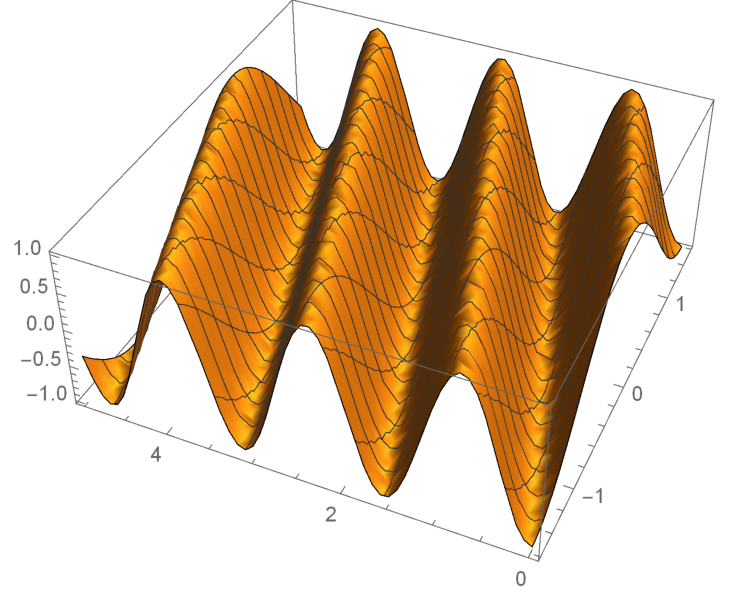
\includegraphics[width=3in]{surf_linear_schrodinger}
\end{figure}

\item Consider the equation $w_{tt}=-\nu^2 w_{xxxx}$ with $\nu>0,|x|<\infty$, and $t>0.$ Determine the exact solution subject to the initial conditions $w(x,0)=cos(kx)$ and $w_t(x,0)=k^2\nu sin(kx)$. Discuss the role of the parameters $\nu$ and $k$. Create a surface plot of the solution with $\nu=1,$ and $k=2.$\\

Solution:\\

We begin by making the ansatz $u(x,t)=A\exp(i(kx-\o t)+B\exp(-i(kx-\o t)$. Substituting this into the equation results in two dispersion relations
\bq \o =\nu k^2\;\;\;\;\text{ and }\;\; \o=-\nu k^2\eq 
with wave speeds
$$\frac{\o}{k}=\pm \nu k.$$
Then the parameters $nu$ and $k$ have the same role as in the previous equation. We can then write our solution:
$$w(x,t)=A e^{ik(x-\nu kt)}+Be^{ik(x+\nu kt)}+C e^{-ik(x-\nu kt)}+D e^{-ik(x+\nu kt)}.$$
Applying the initial conditions results in the solution:
\bq w(x,t)=cos(kx+\nu k^2 t).\eq

A surface plot of the real part of the solution is included here:
\begin{figure}[h]
\centering
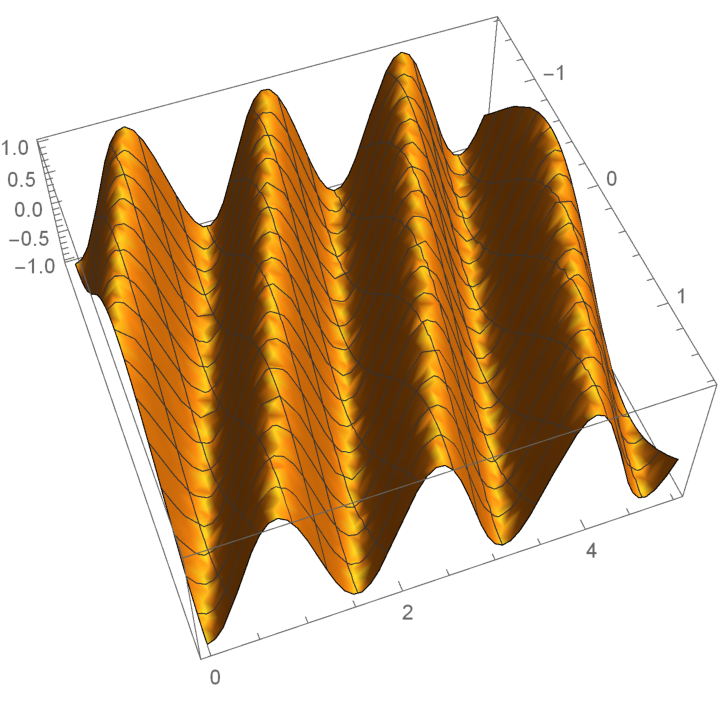
\includegraphics[width=3in]{surf_deriv_lin_schrodinger}
\end{figure}

\item Discuss the relationship between $u$ and $w$ from parts (a) and (b) above.\\

Solution:\\

If we take the time derivative of the equation in part (a), we see
\bq u_{tt}=i\nu u_{xxt}=i\nu(i\nu u_{xx})_{xx}=-\nu^2 u_{xxxx}.\eq
If we look again at the linear Schrodinger equation, we can see that $u=B\exp(-i(kx-\o t))$ is an ansatz with dispersion relation $\o=-\nu k^2.$ Thus we can actually write the solution for this equation as
\bq u(x,t)=Ae^{ik(x-\nu kt)}+B e^{-ik(x+\nu t)}.\eq
Applying the boundary condition clearly requires $B=0$ along with $A=1.$ Thus we see that part of the solution for $w$ is the trivial solution for $u$, and the solution for $u$ is part of the trivial solution for $w$. 


\eenum
\item Consider the equation $u_t=iau_x$ for $a>0,|x|<\infty,t>0.$ Determine the dispersion relation for this equation and discuss the nature of the solutions.\\

Solution:\\

We make the ansatz $u=A \exp(i(kx-\o t))$ to find the dispersion relation for the equation
\bq \o=-i ak.\eq
Then the solutions take the form
\bq u(x,t)=Ae^{ikx}e^{-akt}.\eq
We can see then, that the solutions decay exponentially in time.

\eenum
\pagebreak
The code used to generate the text in problems 1-3 is included here.
\begin{itemize}
\item MATLAB code
\begin{lstlisting}

fprintf('HELLO FROM MATLAB \n');

for i=1:10
    fprintf('%1i %4.6e %4.6e \n',i,1/i,sin(1/i));
end
\end{lstlisting}

\item C code
\begin{lstlisting}
#include<stdio.h>
#include<math.h>

double main()
{
     int count;
     double z, y, x;
     printf("HELLO FROM C\n");
     for(count = 1; count<11; count++)
     {
          z=count;
          x=1/z;
          y=sin(x);
          printf("%d %lf %lf\n",count,x,y);
     }
return 0;
}
\end{lstlisting}

\item FORTRAN code
\begin{lstlisting}
      program problemSet1Fortran
	 
	 integer i, n
	 real y
	 write(*,*) 'HELLO FROM FORTRAN'
	 do 10 i = 1, 10
          y=i
          write(*,*) i,'', 1/y,'', sin(1/y)
10    continue

      end
\end{lstlisting}
\end{itemize}
\end{document}